\documentclass{article}
\usepackage{a4wide}
\usepackage{norsk}
\usepackage{amsmath}
\usepackage{amssymb}
\usepackage{dsfont}
%\usepackage[dvips]{epsfig}
%\usepackage{graphicx}
\usepackage{fancyhdr}
\usepackage{listings}
\usepackage{nomencl}
\usepackage[pdftex]{graphicx}

\pagestyle{fancy}
\lhead{\footnotesize \parbox{11cm}{Andreas Johann H\"ormer (753179)}}
\rhead{\footnotesize {Laboratory 2}}
\chead{\footnotesize {TTT4170}}

\title{Report Virtual Sound Sources (Lab 2)}
\author{Andreas Johann H\"ormer}
\date{14.03.2014}

\begin{document}
\thispagestyle{empty}
\maketitle
\thispagestyle{empty}
%\\[5cm]
\begin{center}
TTT4170 Audio Technology\\[3cm]
Lab group:
\begin{itemize}
\item Andreas Johann H\"ormer
\item Milan Stojkovic
\item Andreas Ulvoen\\[3cm]
\end{itemize}
Report delivered: \\[6cm]
FACULTY OF INFORMATION TECHNOLOGY, MATHEMATICS AND ELECTRICAL ENGINEERING\\
NORWEGIAN UNIVERSITY OF SCIENCE AND TECHNOLOGY
\end{center}
\thispagestyle{empty}
\tableofcontents
\thispagestyle{empty}
\newpage
\section*{Summary}
\thispagestyle{empty}
In this laboratory virtual sound sources are handled. Stereo recordings with a xy-stereo microphone pair as well as a recording with a dummy head were made and compared both at loudspeaker and headphone listening. There it can be obtained, that directional hearing is possible with headphones, where the virtual source location can be done easier with the dummy head recording. When using loudspeakers the virtual sound source always has a position between the two loudspeakers. A directional representation of the real sound source is not possible.\\
In an other listening test the influence of sound pressure level differences as well as time delays were obtained. There it can be found out, that the virtual sound source moves to the louder or earlier sound source. A special thing occurs when at time difference listening test. When the time difference gets too big, the two sound sources are obtained as independent ones, a position of a single sound source is not available any more.

\newpage
\setcounter{page}{1}
\section{Introduction}
Hearing is important for our lives. Sound effects like time differences and sound pressure differences let us know the position of a sound source and so avoid us from potential safety risk, e.g. in the car traffic. These differences in SPL, time and spectral behaviour of the signal in the two ears can help to get the right position of the source.\\
In this laboratory the reproducability of sound source positions with different recording techniques was obtained. As recording techniques xy-stereophony as well as binaural recording with using a dummy head were used. The laboratory mainly was done by human perceiving of recorded signals over both loudspeakers and headphones.
\section{Theory}

\section{Measurements}
\subsection{Equipment}
For this laboratory exercise following equipment was used for the measurements:
\begin{itemize}
\item 1 Yamaha Mixing Console (Model: 01v)
\item 1 HDD-Recorder (Model: SoundDevices 722)
\item 2 microphones (Model: Røde NT5)
\item 2 loudspeakers (Model: dynaudio acoustics BM6A)
\item 1 dummy head (Model: KUBii)
\end{itemize}
\subsection{stereo vs. dummyhead recording}
In this task two recordings were made. 
\begin{enumerate}
\item One recording was made with a stereo microphone pair. As recording technique xy-stereophony was used. A person speaking was walking around the microphone in an aequidistant circle.
\item In an other recording the dummyhead was used. A person walked again around the head and speaked.
\end{enumerate}
After this, the two sound recordings were played over headphones and loudspeakers. Following results can be observed:
\paragraph{results\\}
As result it can be obtained that the sound source with dummyhead recording can be located better when it is at the sides and a little bit harder from back and especially when the sound source is in the front. This can be obtained when using headhones. The same is when using the microphone recording, but the ability to locate is more difficult.\\
When listening to the recordings on loudspeakers, locating of the sound source is not possible. The sound source appears always between the two loudspeakers, using the dummyhead recording as well as the microphone recording.
\subsection{sound source deviation SPL}
In this task the position of the virtual sound source regarding to a sound pressure difference between two speakers is measured. Therefore a person speaking was placed in front of a mono microphone and recorded. The reorded signal was played equally strong on two speakers placed in an angle of $60^\circ$. A listener was placed 2 meters in front of the loudspeakers, so that a calculation of the deviation of the virtual sound source from the center between the loudspeakers can easily be calculated with a tan-function. The listening position can be seen in figure \ref{fig:listening}.
\begin{figure}[htbp]
\begin{center}
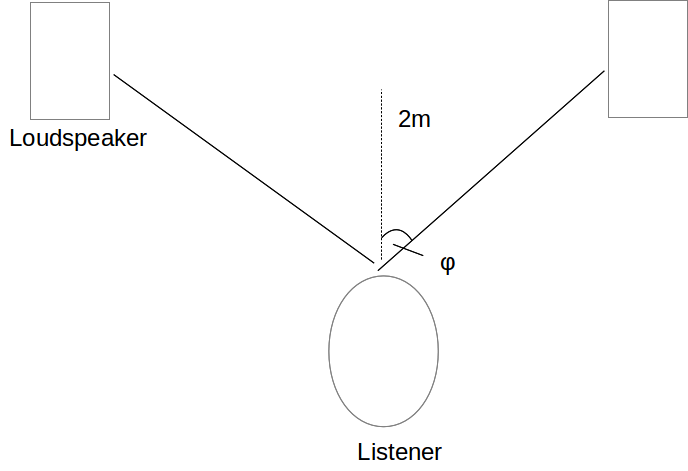
\includegraphics[width=7cm,keepaspectratio=true]{listening}
\caption{Listening position}
\label{fig:listening}
\end{center}
\end{figure}
It can be obtained that with no amplitude difference the sound source appears exactly in the center between the two loudspeakers. With increasing difference of SPL the virtual sound source moves to the speaker with higher sound pressure level. When the sound pressure difference is high enough, the sound is heard as coming only from one speaker. The measured sound source deviation can be seen in table \ref{tab:SPL} as well as in figure \ref{fig:SPL}.
\begin{figure}[htbp]
\begin{center}
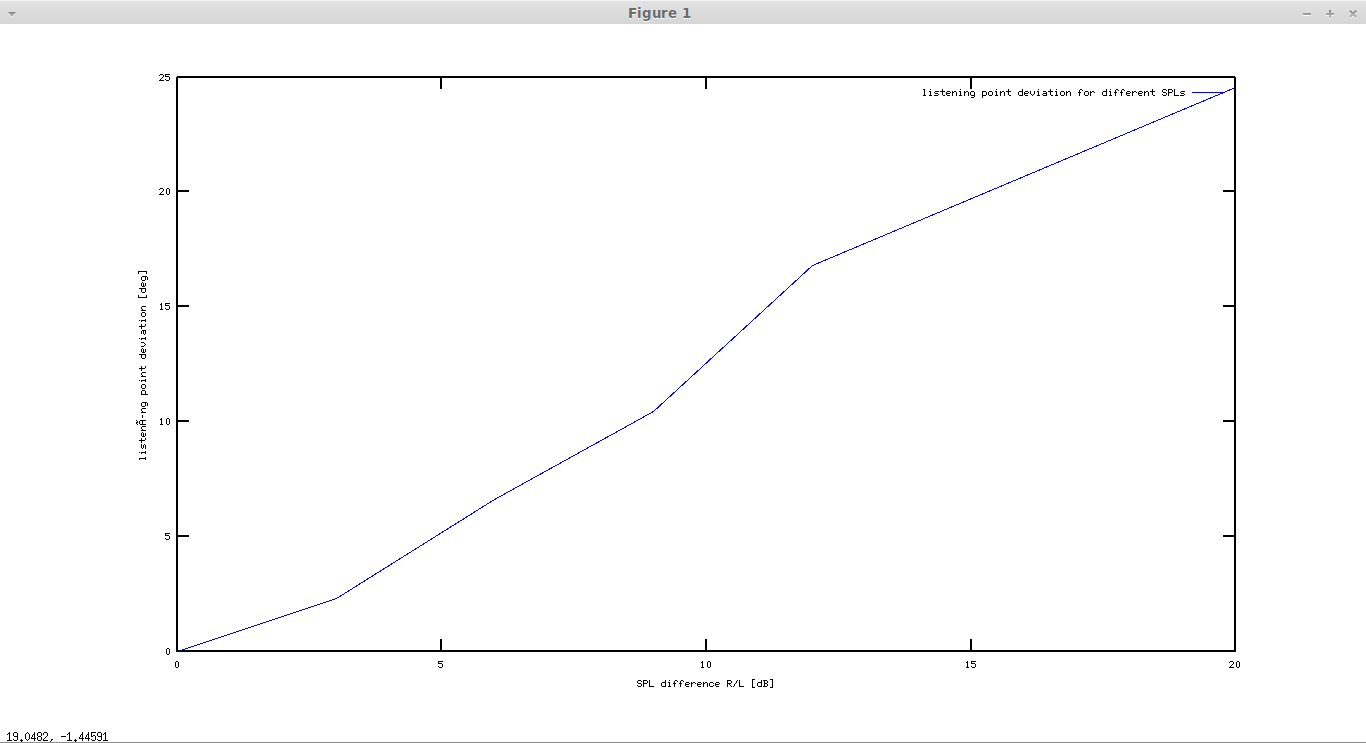
\includegraphics[width=15cm,keepaspectratio=true]{SPL}
\caption{Sound source deviation for different SPLs in degrees}
\label{fig:SPL}
\end{center}
\end{figure}

\subsection{sound source deviation $\Delta t$}
The position of the virtual sound source should be measured with increasing time delay of one loudspeaker. The measured results can be seen in table \ref{tab:time} as well as in figure \ref{fig:timedelay}. Until a certain point is reached, the virtual sound source moves to the speaker which sends the sound first. When the time difference between the two speakers is too big (50ms, 100ms), the two loudspeakers seem as two independent sound sources. In the table the position of the first sound signal occuring is listed for these time delays. 
\begin{figure}[htbp]
\begin{center}
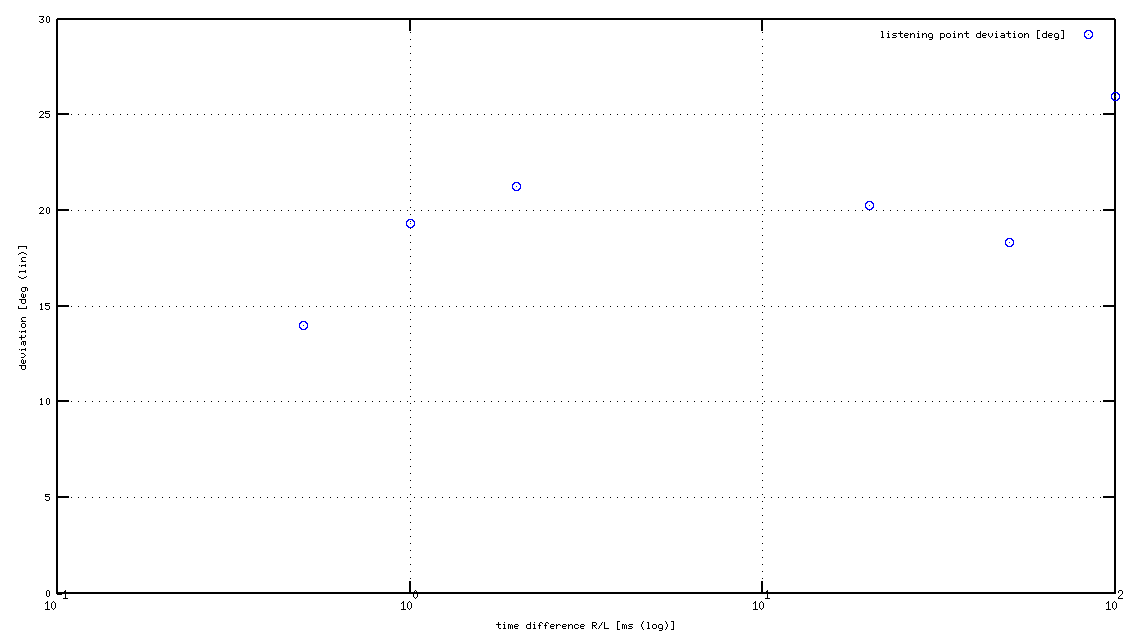
\includegraphics[width=15cm,keepaspectratio=true]{timedifference}
\caption{Sound source deviation for different time differences in ms}
\label{fig:timedelay}
\end{center}
\end{figure}

\begin{table}
\begin{center}
\begin{tabular}{|c||c||c|c|}
\hline
SPL difference & deviation from center & $\phi$ & $\phi$ \\
$dB$	&	$m$	&	$rad$	&	$^\circ$		\\
\hline
\hline
0 & 0 & 0 & 0\\
\hline
3 & 0.08 & 0.04 & 2.29 \\
\hline
6 & 0.23 & 0.116 & 6.62\\
\hline
9 & 0.36 & 0.182 & 10.43\\
\hline
12 & 0.57 & 0.293 & 16.79\\
\hline
20 & 0.81 & 0.429 & 24.56\\
\hline
\end{tabular}
\caption{SPL deviation}
\label{tab:SPL}
\end{center}
\end{table}

\begin{table}
\begin{center}
\begin{tabular}{|c||c||c|c|}
\hline
time difference & deviation from center & $\phi$ & $\phi$ \\
$ms$	&	$m$	&	$rad$	&	$^\circ$		\\
\hline
\hline
0 & 0 & 0 & 0\\
\hline
0.5 & 0.28 & 0.245 & 14.02\\
\hline
1 & 0.65 & 0.337 & 19.31\\
\hline
2 & 0.71 & 0.371 & 21.24\\
\hline
20 & 0.68 & 0.354 & 20.27\\
\hline
50 & 0.62 & 0.320 & 18.35\\
\hline
100 & 0.85 & 0.453 & 25.93\\
\hline
\end{tabular}
\caption{time deviation}
\label{tab:time}
\end{center}
\end{table}

\section{Calculations}
\subsection{calculation of $\phi_{SPL}$}
$$\phi_{rad_{3dB}}=tan\bigg(\frac{0.08m}{2m}\bigg)=0.04$$
$$\phi_{deg_{3dB}}=\phi_{rad_{3dB}}\cdot\frac{180^\circ}{\pi}=2.29^\circ$$
$$\phi_{rad_{6dB}}=tan\bigg(\frac{0.23m}{2m}\bigg)=0.116$$
$$\phi_{deg_{6dB}}=\phi_{rad_{6dB}}\cdot\frac{180^\circ}{\pi}=6.62^\circ$$
$$\phi_{rad_{9dB}}=tan\bigg(\frac{0.36m}{2m}\bigg)=0.182$$
$$\phi_{deg_{9dB}}=\phi_{rad_{9dB}}\cdot\frac{180^\circ}{\pi}=10.43^\circ$$
$$\phi_{rad_{12dB}}=tan\bigg(\frac{0.57m}{2m}\bigg)=0.293$$
$$\phi_{deg_{12dB}}=\phi_{rad_{12dB}}\cdot\frac{180^\circ}{\pi}=16.79^\circ$$
$$\phi_{rad_{20dB}}=tan\bigg(\frac{0.08m}{2m}\bigg)=0.429$$
$$\phi_{deg_{20dB}}=\phi_{rad_{20dB}}\cdot\frac{180^\circ}{\pi}=24.56^\circ$$


\subsection{calculation of $\phi_{timedifference}$}
$$\phi_{rad_{0.5ms}}=tan\bigg(\frac{0.28m}{2m}\bigg)=0.245$$
$$\phi_{deg_{0.5ms}}=\phi_{rad_{0.5ms}}\cdot\frac{180^\circ}{\pi}=14.02^\circ$$
$$\phi_{rad_{1ms}}=tan\bigg(\frac{0.65m}{2m}\bigg)=0.337$$
$$\phi_{deg_{1ms}}=\phi_{rad_{1ms}}\cdot\frac{180^\circ}{\pi}=19.31^\circ$$
$$\phi_{rad_{2ms}}=tan\bigg(\frac{0.71m}{2m}\bigg)=0.371$$
$$\phi_{deg_{2ms}}=\phi_{rad_{2ms}}\cdot\frac{180^\circ}{\pi}=21.24^\circ$$
$$\phi_{rad_{20ms}}=tan\bigg(\frac{0.68m}{2m}\bigg)=0.354$$
$$\phi_{deg_{20ms}}=\phi_{rad_{20ms}}\cdot\frac{180^\circ}{\pi}=20.27^\circ$$
$$\phi_{rad_{50ms}}=tan\bigg(\frac{0.62m}{2m}\bigg)=0.320$$
$$\phi_{deg_{50ms}}=\phi_{rad_{50ms}}\cdot\frac{180^\circ}{\pi}=18.35^\circ$$
$$\phi_{rad_{100ms}}=tan\bigg(\frac{0.85m}{2m}\bigg)=0.453$$
$$\phi_{deg_{100ms}}=\phi_{rad_{100ms}}\cdot\frac{180^\circ}{\pi}=25.93^\circ$$

\newpage
\section{Conclusion}

\newpage
\section{Appendix}
\subsection{Example calculations}



\end{document}


